%%% compile it with pdflatex
\documentclass[a4paper]{article}
\usepackage[T1]{fontenc}
\usepackage[utf8]{inputenc}
\usepackage{lmodern}
\usepackage{fancybox}
\usepackage{graphicx}
\usepackage{tabularx}
\usepackage{amssymb}
\usepackage{amsmath}
\usepackage{subfig}

\begin{document}

\title{A Multi-Agent System for\\ playing Briscola Chiamata}
 
\author{Beltran Borja Fiz, Fabrizio De Santis, Marcos Gabarda\\
\small \texttt{\{beltran.borja.fiz, fabrizio.de.santis, marcos.gabarda\}@est.fib.upc.edu}\\
\\
Multi-Agent Systems Course\\
Master in Artificial Intelligence\\
Universitat Polit\`ecnica de Catalunya}
\date{\today}

\newenvironment{fminipage}%
  {\begin{Sbox}\begin{minipage}}%
  {\end{minipage}\end{Sbox}\fbox{\TheSbox}}

\maketitle

\tableofcontents

\newpage

\section{Introduction}\label{sec:intro}

2-APL stands for A Practical Programming Language and is developed at the University of Utrecht as an academic tool for developing intelligent multi-agent systems. With its unique feature of integrating a declarative and an imperative style programming and the ability to use the JADE platform, 2APL is a resourceful platform to program in.

In a previous report\cite{13559521} we described the features of 2APL, along with both formal and operational description of the language. Its tools were presented and a few examples were showcased to see some agents in action. The aim of this report is to present the design and our own prototype of a 2APL multi-agent system to model the card game of Briscola Chiamata. 

There are many features that make Briscola Chiamata an ideal game to model with a multi agent system. The way the game works forces the developer to give agents cooperation, while at the same time being competitive; they have to be reactive, but also proactive; finally they need to also be autonomous and social.

Cooperation in Briscola Chiamata is a double-edge sword, since if you choose the wrong player to cooperate with, you will be the cause of your own defeat. On the other hand, a successful cooperation will most of the time ensure a safe victory. This risk in choosing which players to trust and cooperate with is what makes the game exciting for humans, and hard for agents. Competition is divided into two types, an individual agent competing to win the game alone, and a team of agents, that are unknown for mostly of the game, trying to compete against the opposite team.

Reactivity is an obvious requirement in any card game; when it is your turn to play, you have to play. In Briscola Chiamata however a proactivity is also required since turns are non strict, i.e: a player can decide to play outside his turn to cheat others of not being interested in the current round or exchange information with other players. This freedom of the game needs to be given to the agents.

The social factor comes from the fact that teams are created without the agents knowing who they are partners and this creates the necessity for communication between them in order to try to determine who are their partners. This, of course, implies a balance between cooperating and cheating. Having agents change status from partner to opponent between rounds makes a dynamic social multi agent system which is worth studying.

The rest of the report is organized as follows. Section~\ref{sec:gamedescr} provides a detailed description of the game. Section~\ref{sec:sysspec},~\ref{sec:highdesign},~\ref{sec:detaildesign} respectively introduces the system specification, architectural design and detailed design of our system following the \emph{Prometheus} design methodology. Finally, we display the built prototype in Section~\ref{sec:proto} and we conclude the report in Section~\ref{sec:concl} with some remarks, related works and conclusions on the overall success of the prototype.

\section{Game Description}\label{sec:gamedescr}

Briscola Chiamatais the five-player version of the italian game of Briscola\cite{wiki:briscola}. Every player is dealt eight cards, so that no cards remain undealt. Then, each player, starting from the dealer's right\footnote{If the dealer is not one the players, then starting from the declearer's right.} and proceeding counter-clockwise, bids in an auction to declare how many points they will score. A player may pass, and hence cannot bid again in that game. The bid represents the number of points that player believes he is capable of accumulating. Bidding continues until all but one player have passed in a round. This remaining player has then ``won the bid'' and therefore gets to declare the Briscola. The declarer also declares a specific Briscola card (example, the ``Ace of Cups'') and the holder of this card is then determined to be the declarer's partner. Logically, the declarer would declare the highest Briscola card he does not already hold in the hopes of creating the strongest combined hand between him and his partner.
The remaining three players are partnered with each other, without their knowledge. Each player, other than the declarer's partner, acts independently, until it is clear which players are partners. Infrequently, the declarer may declare a Briscola card he already holds (if he feels he has a very strong hand), in which case the other four players are partnered against him.
Game strategy is often devised to determine which player is partnered with the declarer, whereas the declarer's partner may devise ruses and decoy strategies to fool the other players, such as not taking a trick, or playing points on a trick that will be won by an opponent.

\paragraph{Scoring}

Each player collects tricks as per the regular version of the game, and counts points collected similarly. Partners, which are known by the end of the game (when briscola card is dealt), then combine their points. Game points are assigned as follows: if the declarer and partner accumulate card points greater than or equal to the points that were declared after the bidding process, then the declarer earns two game points, the partner earns one game point and the other players each lose one game point. If the declarer and partner accumulate fewer card points than declared, then  the declarer loses two game points, the partner loses one game point and the other players each earn one game point. These points are accumulated after every game. The grand winner is the player with the most points at the end of the last match. Note that if the declarer calls a Briscola he holds, then the declarer will win or lose four points, and every other player will win or lose one point.

\section{System Specification}\label{sec:sysspec} 

According to Prometheus methodoly, in the system specification phase, the actors expected to interact with the system, are identified, along with the interface to the system in terms of actions and percepts; system goals are elaborated, and scenarios described in terms of sequences of steps are developed. Roles encompassing small chunks of functionality (identified by goals, percepts and actions) are described and captured.

\subsection{Analysis Overview Diagram}

The analysis overview diagram is designed to show the interactions between the system and the environment. At this abstract level it is necessary to identify the actors, scenarios, percepts and actions involved in the system. This consists of a two step process. Firstly, we identify the actors and the scenarios they participate in with the system. Secondly, we identify and define the actions and percepts between the actors and the system. 

The only actor we felt to model in this first sketch of our game is the user of the system that can be either human or software. Here follows a brief description of each of the scenarios we have identified for it: 
\begin{itemize}
  \item ``Start the game Scenario'' is in charge of receiving join requests from users and accept and subscribe users or queue their requests. Once there are 5 players registered in the system.
  \item ``Dealing scenario'' is in charge of choosing the dealer, shuffle the deck and deal cards to all subscribed the players in the system. 
  \item ``Bidding scenario'' takes place once the dealing is over. It is in charge of giving players a chance to bid. The player who wins the bid, must declare the Briscola card. If nobody bids, then the game has to be restarted. If the bidding succeeds, the Briscola card is declared by the winner of the bid.
  \item ``Play the game'' scenario occurs once all bids are over and the game finally starts. The team distributions are obviously unknown to all players until the Briscola card is played. The players have to update their beliefs about the team distributions each time a card is played. Of course, cheating is part of the game. Communication that is used to model sign exchange among players is allowed to exchange information about players and cards. After each round, points are counted. 
  \item ``End of the game'' scenario is in charge of declaring the winner team, update the score of each player according to the scoring rules and release the player from the system. 
\end{itemize}

Finally, percepts in the system and their consequent actions are summarized in Table~\ref{table:inout}.

\begin{table}[htp]
  \centering
  \begin{tabular}{|l|l|}
    \hline
    Join request	& Subscribe user and manage request  \\
    \hline
    5 players subscribed	& Choose the card dealer \\
    \hline
    Dealer identified	& Shuffling and dealing cards  \\
    \hline
    Deal is over	& Select turn \\
    \hline
    Turn selected	& Declare bid \\
    \hline
    Bid is over	& Declare Briscola card \\ 
    \hline
    Briscola card	& Select turn  \\
    \hline
    Turn selected	& Play card  \\
    \hline
    Card played	& Select turn\\
    \hline
    No percepts needed & Exchange information \\
    \hline
    Round is over	& Count points \\
    \hline
    Game is over	& Declaring the winner \\
    \hline
    Winner declared	 & Update the scoring \\
    \hline
    Scoring updated	& Release the players \\
    \hline
  \end{tabular}
  \label{table:inout}
  \caption{Summary of percepts and actions in the system}
\end{table}


\begin{figure}[htp]
  \centering
  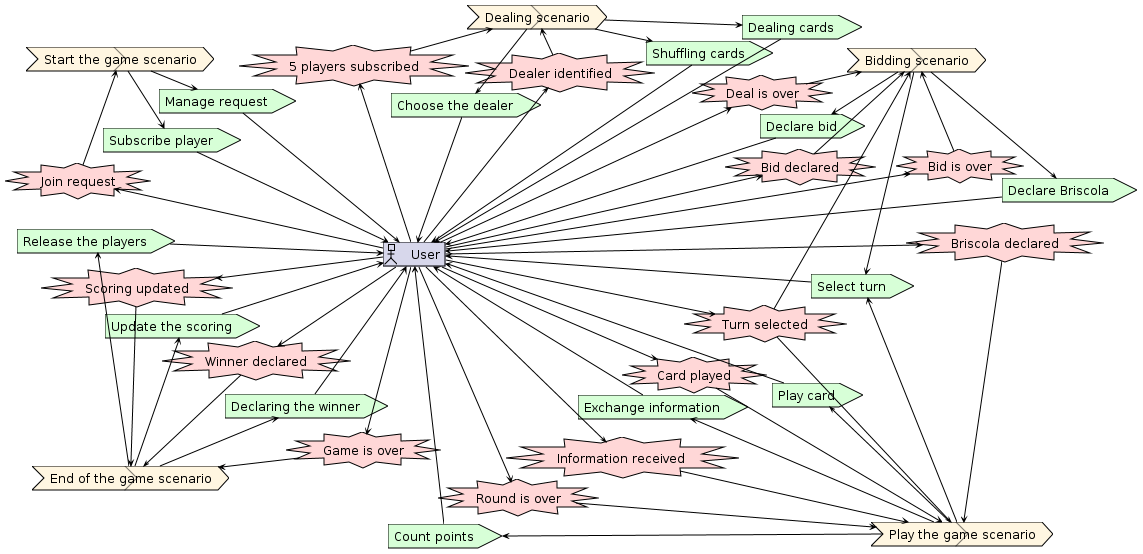
\includegraphics[keepaspectratio,scale=0.35]{pdt/images/system_specification/analysis_overview.png}
  \label{fig:analysis}
  \caption{Analysis overview diagram}
\end{figure}

Figure~\ref{fig:analysis} provides the analysis overview diagram for our game.


\subsection{Scenarios Diagram}

The scenarios cover all the phases of the game shows the dynamics of the game. First, the ``start the game scenario'' waits for players to register in the system, then the ``dealing scenario'' deals cards to the players, after that the ``bidding scenario'' allows the players to do their bids, then ``play the game scenario'' allows them to play the game and finally the ``end the game scenario'' assigns them their score. If nobody of the players leave the system, another game can be started, again from the ``dealing scenario''. The scenarios diagram is provided in Figure~\ref{fig:scenarios} .

\begin{figure}[htp]
  \centering
  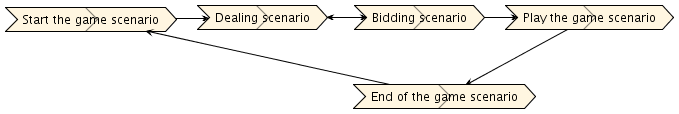
\includegraphics[keepaspectratio,scale=0.5]{pdt/images/system_specification/scenarios.png}
  \label{fig:scenarios}
  \caption{Scenarios diagram}
\end{figure}

\subsection{Goals Diagram}

The goal overview diagram is a directed acyclic graph of all goals in the system showing how goals can be decomposed into subgoals. Sub-goals can be generated by asking ``how will the system accomplish this goal'' while parent goals can be generated by asking ``why does the system accomplish this goal''. Figure~\ref{fig:goals} shows our goals diagram for the game.

\begin{figure}[htp]
  \centering
  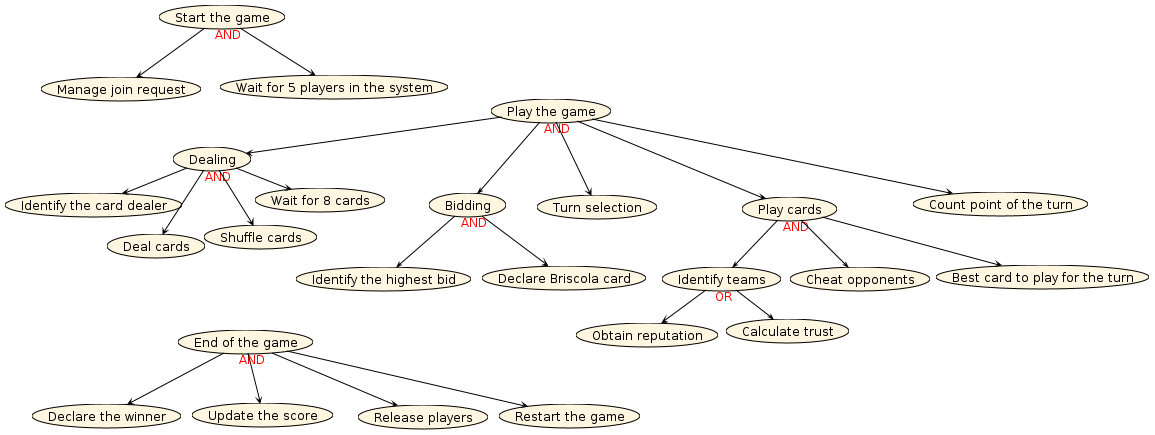
\includegraphics[keepaspectratio,scale=0.4]{pdt/images/system_specification/goal_overview.png}
  \label{fig:goals}
  \caption{Goals diagram}
\end{figure}
  
\subsection{System Roles Diagram}

In the system roles diagram, we group different goals, percepts and actions under roles. This helps in further modularizing the system into functionality. The input is represented as a percept and the output as an action. Figure~\ref{fig:sysroles} shows our system roles diagram for the game. Each role should be limited in scope, and be able to be described fully be 1-2 sentences. According to this principle, here follows the descriptions we have identified:
\begin{itemize}
  \item ``Starting game role'' manages the join requests
  \item ``Identify the dealer role'' identifies who is the dealer in the game
  \item ``Dealing role'' shuffle and deal cards to the players
  \item ``Bidding role'' manage bids
  \item ``Declaring Briscola role'' declares the Briscola card
  \item ``Turn control role'' decides player's turn to play
  \item ``Playing role'' play a strategy
  \item ``Team setting role'' try to infer team settings
  \item ``Counting points role'' counts points of each round
  \item ``Declare the winner role'' declares the winner team of the game
  \item ``Update score points'' updates the score board 
  \item ``Release the player'' release the players from the game
\end{itemize} 

\begin{figure}[htp]
  \centering
  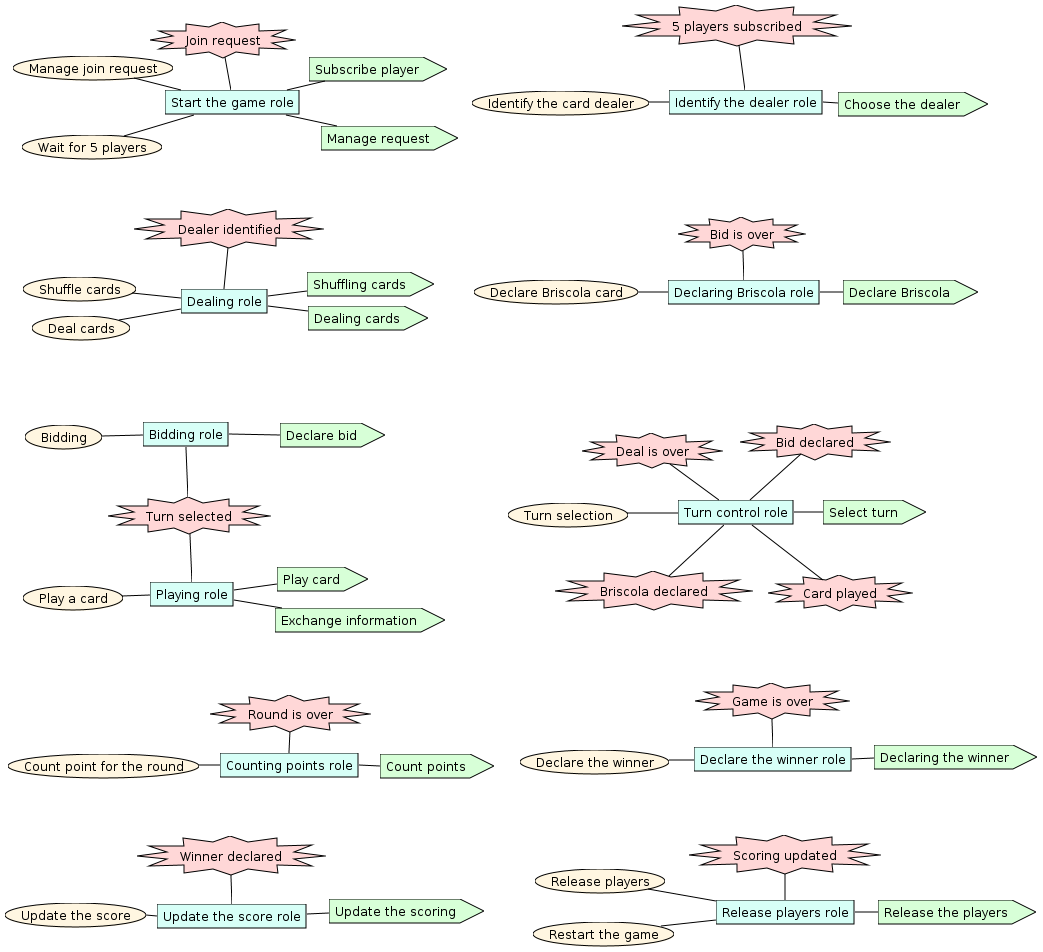
\includegraphics[keepaspectratio,scale=0.4]{pdt/images/system_specification/system_roles.png}
  \label{fig:sysroles}
  \caption{System roles diagram}
\end{figure}

\newpage 

\section{Architectural Design}\label{sec:highdesign}

In this phase, the agent types that will exist in the system are defined by combining roles, the overall structure of the system is described using a system overview diagram, and interaction protocols are used to capture the dynamics of the system in terms of legal message sequences.

\subsection{Data Coupling Diagram}

The roles that were formed in the last step of the previous phase are linked to data that has been identified as necessary for performing that role. Here follows the list of the data types that have been identified in the system: 
\begin{itemize}
  \item ``Position'' that record the position of the player at the table that is useful to decide its turn
  \item ``Deck'' that contains all the cards
  \item ``Hand'' that represents the cards in hand of each player
  \item ``Historic of bids'' that records the historic of bids
  \item ``Historic of card played'' that analogously records the historic of card played in order to decide which card to play
  \item ``Team information'' that is used to store beliefs about team settings
  \item ``Points'' that is used to store the points of each round
  \item ``Scoreboard'' that contains the all the times score of the games for each player. 
\end{itemize}

The data coupling diagram is provided in Figure~\ref{fig:datacoupl}.

\begin{figure}[htp]
  \centering
  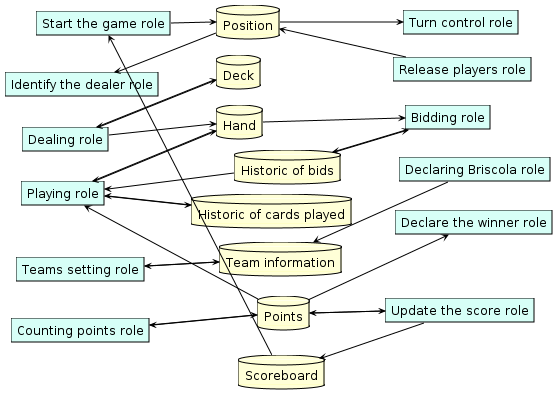
\includegraphics[keepaspectratio,scale=0.45]{pdt/images/architectural_design/data_coupling.png}
  \label{fig:datacoupl}
  \caption{Data coupling diagram}
\end{figure}

\subsection{Agent-Role Grouping Diagram}

In this diagram we group the roles into agent types. The agent-role coupling diagram shows the group of roles that come under an agent. Here follows the list of the agent types that we have indentified:
\begin{itemize}
  \item ``Dealer'' that is the that represents the dealer that is in charge of dealing cards
  \item ``Gatekeeper'' that is the that represents the agent that let the players come in and out the system
  \item ``Non-player charcter'' that is the that represents the actual players in the system
  \item ``Notary'' that is the that agent type represents the agent in charge of controlling the game
\end{itemize}

Figure~\ref{fig:agentrole} provides the agent-role grouping diagram for our game.

\begin{figure}[htp]
  \centering
  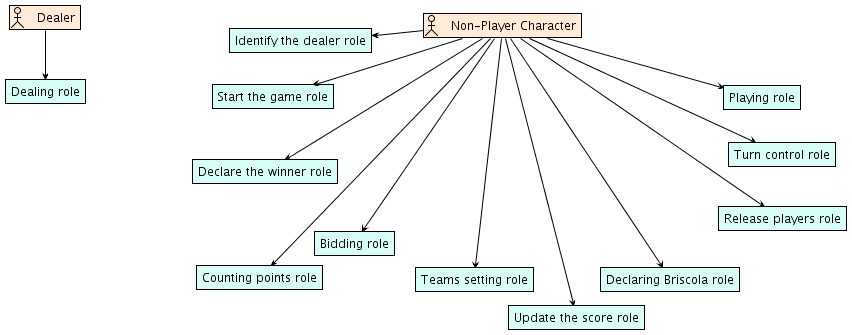
\includegraphics[keepaspectratio,scale=0.45]{pdt/images/architectural_design/aget-role_grouping.png}
  \label{fig:agentrole}
  \caption{Agent-role grouping diagram}
\end{figure}

\subsection{Agent Acquaintance Diagram}

In the agent acquaintance diagram you can see all agents within the system and which agents interact. The agent acquaintance diagram is provided in Figure~\ref{fig:agentacq}. 

\begin{figure}[htp]
  \centering
  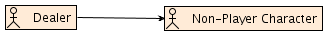
\includegraphics[keepaspectratio,scale=0.45]{pdt/images/architectural_design/agent_acquaintance.png}
  \label{fig:agentacq}
  \caption{Agent acquaintance diagram}
\end{figure}

\subsection{System Overview Diagram}

In the system overview diagram you can see all agents in the system, along with their interface and interactions. The system overview diagram is provided in Figure~\ref{fig:sysovervw}.

\begin{figure}[htp]
  \centering
  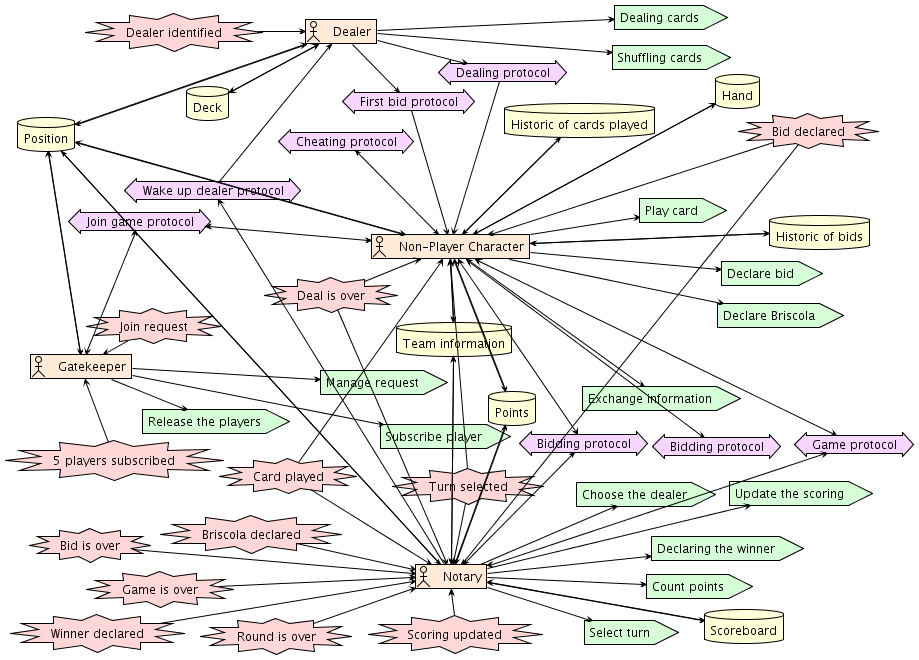
\includegraphics[keepaspectratio,scale=0.45]{pdt/images/architectural_design/system_overview.png}
  \label{fig:sysovervw}
  \caption{System overview diagram}
\end{figure}

\section{Detailed Design}\label{sec:detaildesign}

In this phase, the internals of each agent are developed in terms of capabilities, events, plans and data at the level of individual agents.

\subsection{Agent Overview Diagram}
The agent overview diagram shows the internals of an agent. Thus, there is one agent overview diagram for every agent in the system: the dealer, the gatekeeper, the 5 non-player character and the notary. Their diagrams are respectively provided in Figure~\ref{fig:dealer}, Figure~\ref{fig:notary}, Figure~\ref{fig:gatekeeper} and Figure~\ref{fig:nonplay-char}.

\begin{figure}[htp]
  \centering
  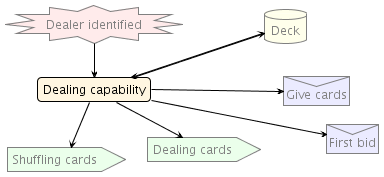
\includegraphics[keepaspectratio,scale=0.45]{pdt/images/detailed_design/dealer_overview_diagram.png}
  \label{fig:dealer}
  \caption{Agent overview diagram for the dealer agent}
\end{figure}
\begin{figure}[htp]
  \centering
  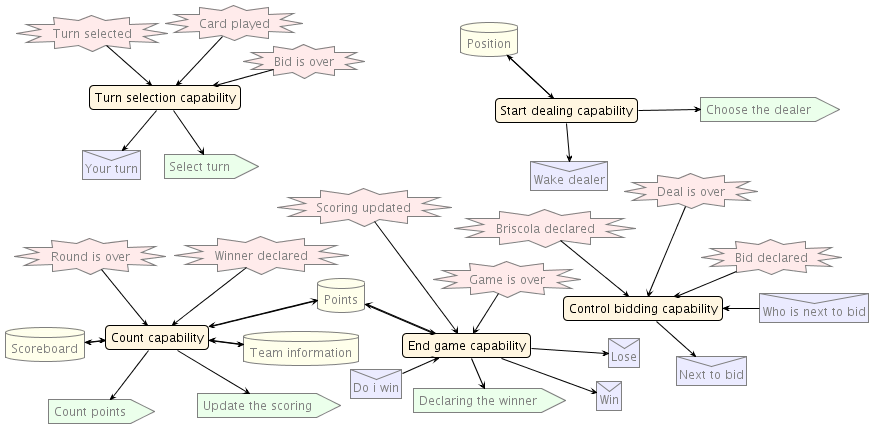
\includegraphics[keepaspectratio,scale=0.45]{pdt/images/detailed_design/notary_overview_diagram.png}
  \label{fig:notary}
  \caption{Agent overview diagram for the notary agent}
\end{figure}
\begin{figure}[htp]
  \centering
  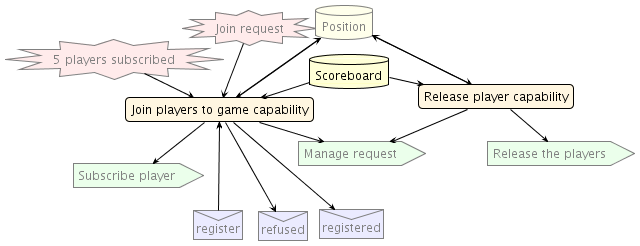
\includegraphics[keepaspectratio,scale=0.45]{pdt/images/detailed_design/gatekeeper_overview_diagram.png}
  \label{fig:gatekeeper}
  \caption{Agent overview diagram for the gatekeeper agent}
\end{figure}
\begin{figure}[htp]
  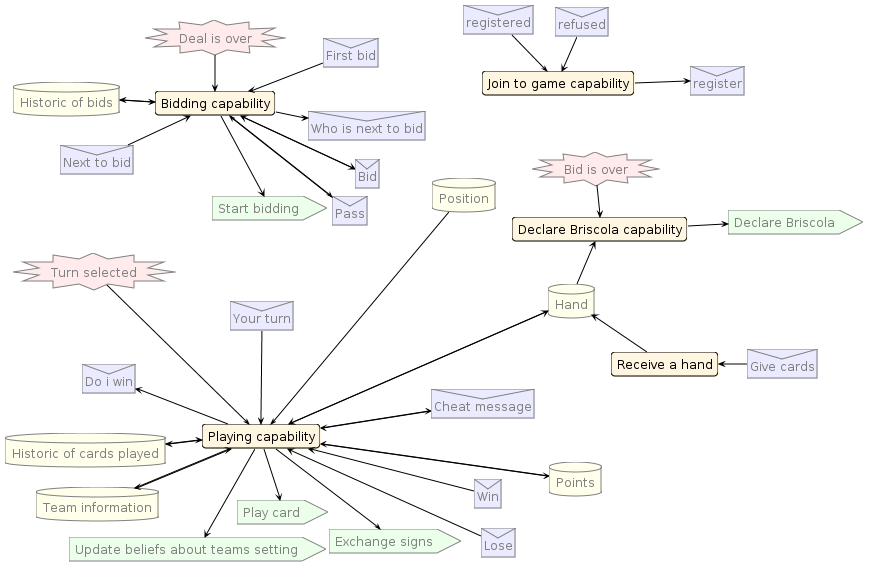
\includegraphics[keepaspectratio,scale=0.45]{pdt/images/detailed_design/non-player_character_overview_diagram.png}
  \label{fig:nonplay-char}
  \caption{Agent overview diagram for the non-player character agent}
\end{figure}
  

\subsection{Capability Overview Diagram}
The capability overview diagram allows to specify the internals of a capability in terms of plans, or sub-capabilities and messages between them for each agent. Figure~\ref{fig:dealing-cap} provides the capabilities for the dealer agent, Figure~\ref{fig:notary-cap} for the notary agent, Figure~\ref{fig:gatekeeper-cap} for the gatekeeper agent and Figure~\ref{fig:non-player-cap} for the non-player character agent, 

\begin{figure}[htp]
  \centering
  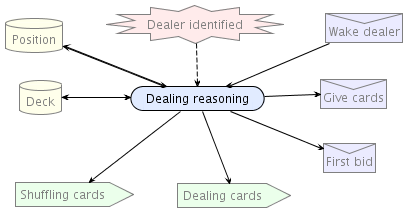
\includegraphics[keepaspectratio,scale=0.45]{pdt/images/detailed_design/dealing_capability_overview_diagram.png}
  \label{fig:dealing-cap}
  \caption{Capability overview diagram for capabilities of the dealer agent}
\end{figure}
\begin{figure}[htp]
  \centering
  \subfloat[Turn selection]{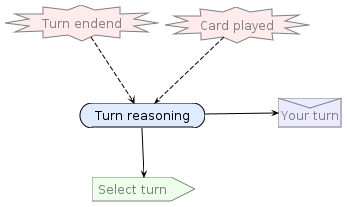
\includegraphics[keepaspectratio,scale=0.45]{pdt/images/detailed_design/turn_selection_capability_overview_diagram.png}}
  \subfloat[End the game]{
\includegraphics[keepaspectratio,scale=0.45]{pdt/images/detailed_design/end_the_game_capability_overview_diagram.png}}\\
  \subfloat[Start dealing]{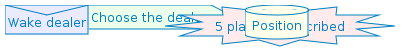
\includegraphics[keepaspectratio,scale=0.45]{pdt/images/detailed_design/start_dealing_capability_overview_diagram.png}}
  \subfloat[Control bidding]{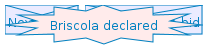
\includegraphics[keepaspectratio,scale=0.45]{pdt/images/detailed_design/control_bidding_capability_overview_diagram.png}}\\
  \subfloat[Count points]{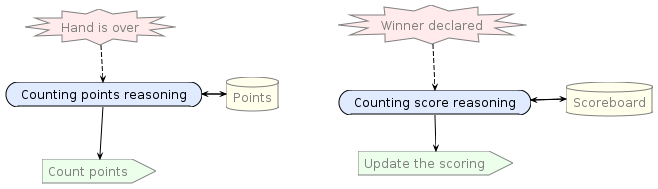
\includegraphics[keepaspectratio,scale=0.45]{pdt/images/detailed_design/count_points_capability_overview_diagram.png}}
  \label{fig:notary-cap}
  \caption{Capability overview diagram for capabilities of the notary agent}
\end{figure}
\begin{figure}[htp]
  \centering
  \subfloat[Release player]{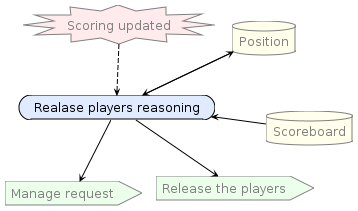
\includegraphics[keepaspectratio,scale=0.45]{pdt/images/detailed_design/release_player_capability_overview_diagram.png}}
  \subfloat[Join players]{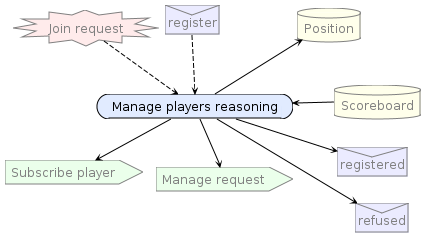
\includegraphics[keepaspectratio,scale=0.45]{pdt/images/detailed_design/join_players_capability_overview_diagram.png}}
  \label{fig:gatekeeper-cap}
  \caption{Capability overview diagram for capabilities of the gatekeeper agent}
\end{figure}
\begin{figure}[htp]
  \centering
  \subfloat[Receive hand]{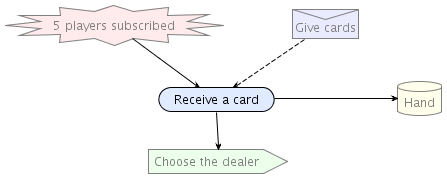
\includegraphics[keepaspectratio,scale=0.45]{pdt/images/detailed_design/receive_a_hand_capability_overview_diagram.png}}
  \subfloat[Bidding]{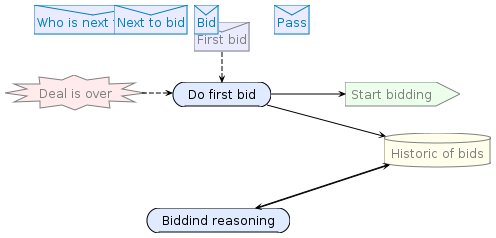
\includegraphics[keepaspectratio,scale=0.45]{pdt/images/detailed_design/bidding_capability_overview_diagram.png}}\\
  \subfloat[Playing]{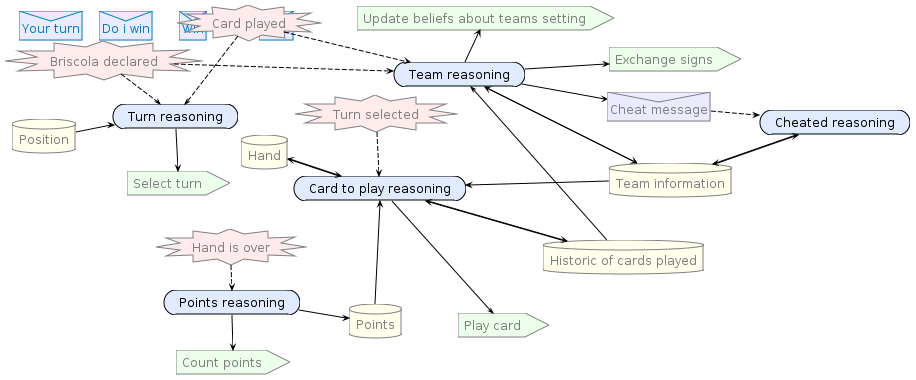
\includegraphics[keepaspectratio,scale=0.45]{pdt/images/detailed_design/playing_capability_overview_diagram.png}}\\
  \subfloat[Declare briscola]{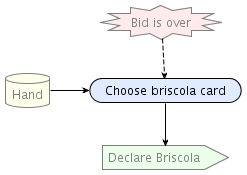
\includegraphics[keepaspectratio,scale=0.45]{pdt/images/detailed_design/declare_briscola_capability_overview_diagram.png}}
  \subfloat[Join the game]{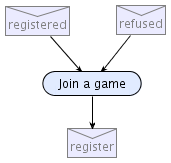
\includegraphics[keepaspectratio,scale=0.45]{pdt/images/detailed_design/join_to_game_capability_overview_diagram.png}}
  \label{fig:non-player-cap}
  \caption{Capability overview diagram for capabilities of the non-player character agent}
\end{figure}

\section{Prototype}\label{sec:proto} 

The prototype was built according the design decisions as described in the previous sections, each step was carefully defined, built and implemented. % The idea was to use as many features as 2APL as possible, and thus our own personal environment was also created for this Paper.
The development of the prototype can be logically separated in two parts: firstly the environment in which the agents interact, and secondly the agents themselves.

Environments in 2APL, as mentioned in the previos paper, are created as a Java class extension. By using the example environment given in the documentation of 2APL we were able to build our own environment adding it a graphic user interface (GUI) to allow monitoring visually the agents in action. This environment was built so that it would allow agents to interact in all of the possible manners defined during the design stage. We successfully implemented it with a GUI that achieved the desired level of detail as to be pleasing to the eye but not a burden to the real task at hand: the way the agents act and interact. A screen shot of the GUI is provided in Figure~\ref{fig:gui1}. As you can see it was decided to split the GUI into three panels: the left panel being the one which shows each players cards, score and bid; a top right corner in which cards played are shown, and a bottom right panel in which information about the agent interactions is displayed, along with game information. Teams are highlighted in different colors, black and blue.

\begin{figure}[htp]
  \centering
  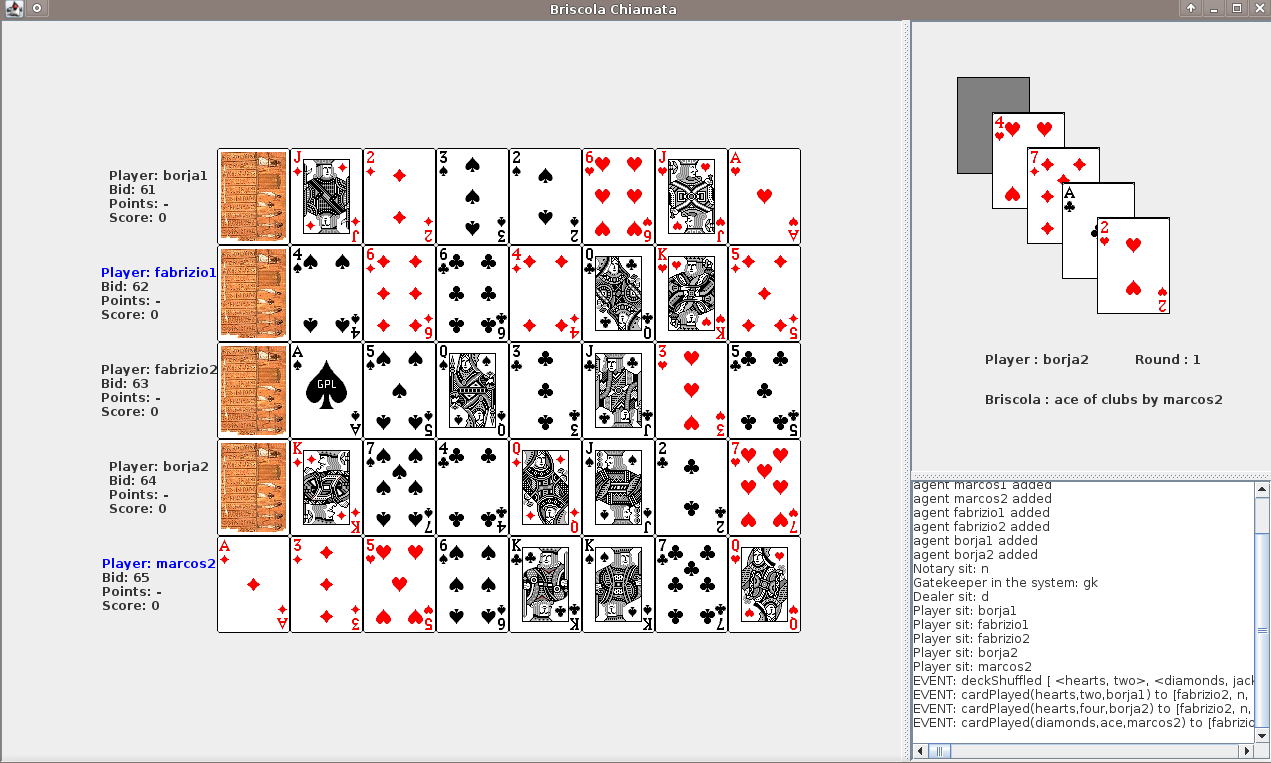
\includegraphics[keepaspectratio,scale=0.3]{fig/gui1.png}
  \label{fig:gui1}
  \caption{Screenshot from the graphical user interface}
\end{figure}

%The agents were designed separately using prolog, and saved in separate files depending on the strategy they were programmed to have.
Since there are five players in a Briscola Chiamata game, we were able to have up to five agents having different strategies fighting against each other and we would be able to see the victorious strategy. 
%Even though Prolog is mainly used to create the agent, it is of limited use in the belief base and the usage of extra libraries could give the user more freedom when designing them (and  stronger strategies too).

The prototype however, as its name indicates, is merely a prototype and thus implements the most simplistic aspects . The agents were implemented to follow straight forward strategies with very little cooperation and even ``cheating'' in order to find their partners during a game round. It is worth mentioning that during the testing part, the 2APL parser was in most cases completely useless as the error messages it provides as feedback are unclear and unhelpful. This makes the task of perfectioning the prototype hard and tedious. %Finally it is worth mentioning that this prototype was built so that it could easily be extended. For example it could be extended into an application which accepts both human and agent players, and even further to be played using a network and/or the internet in order to fight other agents.

We would have loved to add some of those more advanced features such as having completely radical strategies fighting each other, or even some form of reinforcement learning would have been fantastic to see in action, but time and the difficulty of extending things in 2APL have made it impossible for now.

\section{Conclusion}\label{sec:concl} 

The general feeling after implementing the Briscola Chiamata game into the 2APL system is both good and bad. Let start with the positive aspects.

Having a declarative programming when developing agents certainly gives the designer a certain level of confidence that you would not have with other languages. You can focus specifically on ``what'' you want from your agents to do and not ``how''. This conceptual division is one of the main attractions of 2APL and even though some of us required to learn this type of programming in more depth as we had no previous experience in it, we certainly appreciated the benefit gained when we were in the implementation stage.

The JADE platform tools and some of 2APL tools were certainly helpful from beginning to end and provided us with information that would have otherwise been hard to see or find. Of course we can connect any of our agents to any other agent in the JADE platform and having this kind of openness is a helpful and important feature.

The negative aspects of 2APL are few, but certainly relevant. Firstly it is clearly a tool designed primarily for research and not for industry development. The documentation for 2APL is still relatively vague and requires some updating, while the examples given are few and sadly not fully detailed. The environment and the agents we built were done mostly by scanning the code of the blockworld example and thus we lacked the true ability to implement a full application (this was never our intention, but knowing that implementing a fully operational high scale piece of software would be made harder due to the poor support is worth mentioning).

Even though declarative programming does give us a very powerful logic system, 2APL does lack to provide agents with the capability to compute things on their own. In its current state the designer is forced to have the environment calculate it for the agent, instead of allowing the agent to encapsulate the calculation method in its own code. Finally, even though it was previously mentioned, the 2APL parser was so unhelpful that it barely provided us with any useful information. Clearer instructions or error messages would be necessary if any serious development was to be made in this language.

So even though we praised 2APL for some things and despised it for others, as a whole we were pleased to develop with 2APL and do believe that with more work it can become the ``go to'' language of multiagent systems, at least from a research point of view.


\section{Bibliography}
\nocite{*}
\bibliographystyle{plain}
\bibliography{bc-doc}

\end{document}
